\documentclass{beamer}
%
% Choose how your presentation looks.
%
% For more themes, color themes and font themes, see:
% http://deic.uab.es/~iblanes/beamer_gallery/index_by_theme.html
%
\mode<presentation>
{
  \usetheme{NYU}      % or try Darmstadt, Madrid, Warsaw, ...
  \usecolortheme{default} % or try albatross, beaver, crane, ...
  \usefonttheme{default}  % or try serif, structurebold, ...
  \setbeamertemplate{navigation symbols}{}
  \setbeamertemplate{caption}[numbered]
} 

\usepackage[english]{babel}
\usepackage[utf8x]{inputenc}
\usepackage{pgfpages}
\setbeameroption{show notes}
\setbeamertemplate{note page}[plain]
\setbeameroption{show notes on second screen=right}


\title[Information Sharing for infectious disease]{Information Share for infectious disease}
\author{James Chen}
\institute{NYU Shanghai}
\date{February 7, 2021}
\titlegraphic{\hfill
\includegraphics[height=1.5cm]{nyu_stacked_color}}



\begin{document}
\begin{frame}
  \titlepage
\end{frame}
 \note{
  \point{introduce\\ in this presentation \\ importance \\ how \\ covid}}

% Uncomment these lines for an automatically generated outline.
%\begin{frame}{Outline}
%  \tableofcontents
%\end{frame}

\section{Importance}
\begin{frame}{Importance of information share}
\begin{itemize}

  \item It is critical for information to be shared 
  \item Information can reduce the possibility of the spread of the disease 
  
\begin{figure}[H]
\centering
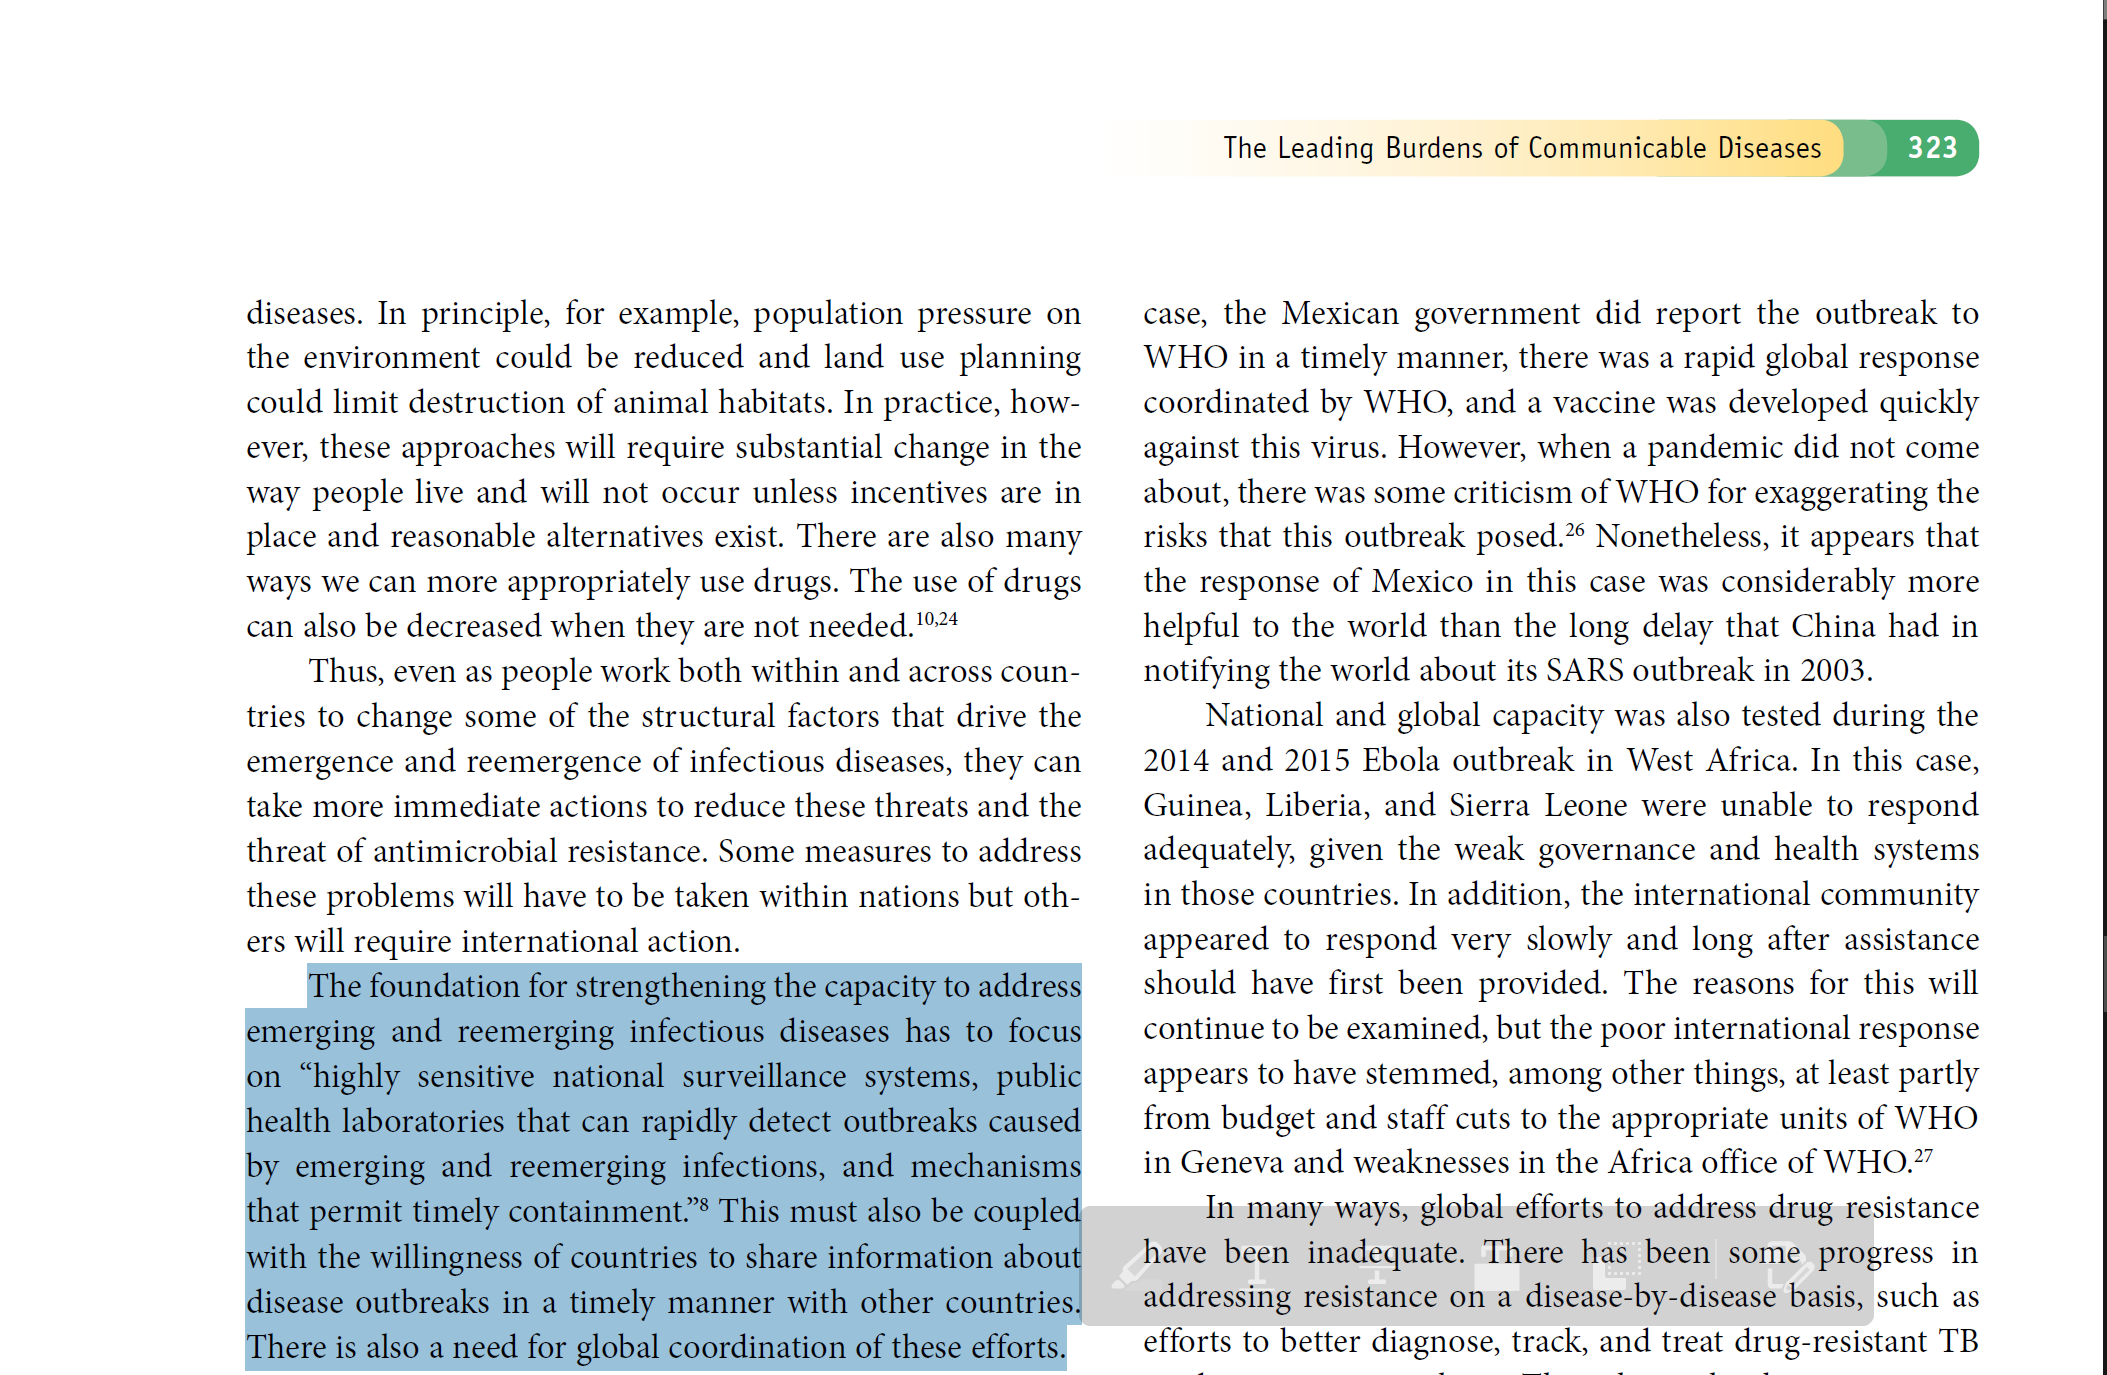
\includegraphics[scale=0.375]{textbook.png}
\caption{The Universe}
\end{figure}
\citep{skolnik_2015}
\end{itemize}
\note{
\point{in textbook\\ if well informed, may stopped at once}
}

\end{frame}



\section{Method}
\begin{frame}{How to share the information and data}
\begin{itemize}

\item Support the World Health Organization.
\item Facilitate the rapid sharing of information during outbreaks.
\item Build greater trust with countries are key to global pandemic preparedness.
\citep{sciencedaily_2017}
\end{itemize}
\note{
\point{published on science daily\\ 2017\\ mainly focus on flu epidmic\\ 1. world leading, the only\\ 2.to build up a framework\\ freely \\ 3.to build trust, get rid of the prejudice \\ignore the difference like political system}
}
\end{frame}


\section{COVID-19}
\begin{frame}{Information share and COVID-19}
\begin{itemize}

\item First confirmed case found in December 2019
\item China shared genetic data to WHO in January 2020
\item Give the foreign scientists possibility to work on the virus before having confirmed case
\note{
\point{in 1 month\\ SARS 5, \\vaccine us china europe russia, 12}
}
\citep{lisa}

\end{itemize}
\end{frame}



\section{Reference}
\begin{frame}[<1>][allowframebreaks]{References}
Schnirring, L. (Ed.). (2020, January 11). China releases genetic data on New coronavirus, now deadly. Retrieved February 03, 2021, from https://www.cidrap.umn.edu/news-perspective/2020/01/china-releases-genetic-data-new-coronavirus-now-deadly\\ \\Sharing of data to combat infectious disease outbreaks. (2017, January 12). Retrieved February 03, 2021, from https://www.sciencedaily.com/releases/2017/01/170112085013.htm\\ \\Skolnik, R. L. (2021). Global health 101. Burlington, MA: Jones &amp; Bartlett Learning.
\note{
\point{greatest in 21\\ a lot of death\\fastest in history\\ hope}
}
\end{frame}

\end{document}
